%!TEX TS-program = xelatex
%!TEX encoding = UTF-8 Unicode

\documentclass[14pt,mathserif]{beamer} 
\usepackage[utf8]{inputenc}
\usepackage{concrete}
%\usepackage{CormorantGaramond}
\usepackage{fontspec}
\usepackage{listings}
\usepackage{amssymb,amsmath}
\usepackage{tabularx}
\usepackage{colortbl}
\usepackage{ifxetex,ifluatex}
\usepackage{fixltx2e} % provides \textsubscript
%\usepackage{lmodern}
\usepackage{natbib}
\usepackage{listings}
\usepackage{framed,graphicx,xcolor}
\usepackage{fancyvrb}
\usepackage{longtable,booktabs}
\usepackage{caption}
\usepackage{url}
\usepackage{graphicx}
\usepackage[normalem]{ulem}
\usepackage{tikz}
\usepackage{semantic}
\usepackage{verbatim}
\usepackage{anyfontsize}
\usepackage{epigraph}
\usepackage{mathtools}
\usepackage[T1]{fontenc}
\let\oldnormalfont\normalfont
\def\normalfont{\oldnormalfont\mdseries}

\usetikzlibrary{positioning,chains,fit,shapes,calc}
\usefonttheme{serif}
\setromanfont{CormorantGaramond}[Numbers={,Lining}]
\setmathrm{CormorantGaramond}[Numbers={,Lining}]
\setmonofont{Inconsolata}

\lstset{basicstyle=\ttfamily,frame=none}

\usenavigationsymbolstemplate{}
\setbeamertemplate{footline}{}
\setbeamertemplate{headline}{}
\graphicspath{ {pics/} }

\definecolor{red}{RGB}{186,12,47}
\definecolor{grey}{RGB}{99,102,106}

\setbeamerfont{structure}{family=\rmfamily, shape=\scshape}
\setbeamercolor{structure}{fg=red}
\setbeamercolor{normal text}{fg=grey,bg=white}
\setbeamerfont{normal text}{family=\rmfamily}

\defbeamertemplate{itemize item}{image}{$\circ$}
\setbeamertemplate{itemize item}[image]

\def\ce{$\mathcal{\mathcal{C} \mskip -1mu \mathcal{E}} \mskip 4mu$}

\newcommand{\sectionslide}[3]{
  \begin{frame}
  \vspace{1cm}
  \vfill
  {\usebeamerfont{title} \color{red} #1}
  \vfill
  \epigraph{\footnotesize{#2}}{\footnotesize{\emph{#3}}}
  \end{frame}}

\title{Shared-Environment Call-by-Need}
\author{George Stelle}
      
\institute{
\includegraphics[width=0.3\columnwidth]{unm.pdf}}
\date{}
\begin{document}
\frame{\titlepage}

\begin{frame}
\frametitle{Outline}
\begin{itemize}
\item Introduction 
\item \ce Machine
\item Native Code Compilation
\item Verified Compilation
\item Conclusion
\end{itemize}
\end{frame}

\sectionslide{Introduction}
{Functional programming combines the flexibility and power of abstract
mathematics with the intuitive clarity of abstract mathematics.}
{Randall Munroe (xkcd)}

\begin{frame}
\frametitle{Lambda Calculus}
$$t \Coloneqq x \; | \; \lambda x.t \; | \; t \; t$$
\end{frame}

\begin{frame}
\frametitle{De Bruijn Indices}
\begin{align*}
i &\in \mathbb{N} \\
t &\Coloneqq i \; | \; \lambda t \; | \; t \; t
\end{align*}
\begin{align*}
\lambda 0 &\equiv \lambda x.x \\
\lambda \lambda 1 &\equiv \lambda x.\lambda y.x
\end{align*}
\end{frame}

\begin{frame}
\frametitle{Call-by-need (Lazy)}
\begin{itemize}
\item Only evaluate when necessary
\item Never evaluate more than once
\end{itemize}
\end{frame}

\begin{frame}{Evaluation Strategies}
\begin{center}
Call-by-Value: $\{1\}$ \\ 
Call-by-Name: $\mathbb{N}$ \\ 
Call-by-Need: $\{0,1\}$
\end{center}
\end{frame}

\begin{frame}[fragile]
\frametitle{Example}
\begin{lstlisting}
doubleOrNothing b x = if b 
  then x + x
  else 0

doubleOrNothing 
  (decisionProblem y) 
  (expensiveComputation z)
\end{lstlisting}
\end{frame}

\begin{frame} 
\frametitle{Laziness}
[L]azy functional programming is too important to be relegated to second-class
citizenship. It is perhaps the most powerful glue[.]

\null\hfill \emph{John Hughes}
\end{frame}

\begin{frame}
\frametitle{Motivation}
\large
\begin{center}
Performance 
\\
\null\hfill
\\
Correctness
\end{center}
\end{frame}

\begin{frame}[fragile]
\frametitle{Environment Representation}
\begin{lstlisting}[frame=single]
f (g x y z) 
  (h w x y z)
\end{lstlisting}
\begin{figure}
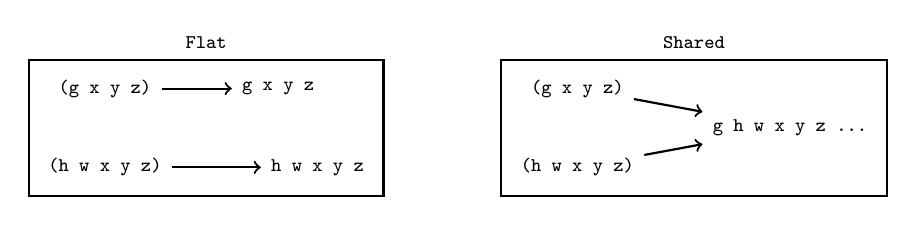
\begin{tikzpicture}[thick,->]
\tikzstyle{every node}=[font=\scriptsize\ttfamily]
% the vertices of U
\begin{scope}[xshift=0cm]
\node (g) {(g x y z)};
\node[right of=g, node distance=2.2cm] (genv) {g x y z};
\node[below of=g] (h) {(h w x y z)};
\node[right of=h, node distance=2.7cm] (henv) {h w x y z};
\draw (g) -- (genv);
\draw (h) -- (henv);
\end{scope}
\node [fit=(g) (genv) (h) (henv),label=above:Flat,rectangle,draw] (flat) {};
\begin{scope}[xshift=6cm]
\node (g') {(g x y z)};
\node[below of=g'] (h') {(h w x y z)};
\node[right of=h', node distance=2.7cm, yshift=5mm](env) {g h w x y z ...};
\end{scope}
\draw (g') -- (env);
\draw (h') -- (env);

\node [fit=(g') (h') (env),label=above:Shared,rectangle,draw] {};
\end{tikzpicture}
\end{figure}
\end{frame}

\begin{frame}[fragile]
\frametitle{Strictness}
\begin{lstlisting}
doubleOrNothing b x = if b 
  then x + x
  else 0

doubleOrNothing 
  (decisionProblem y) 
  (expensiveComputation z)
\end{lstlisting}
\end{frame}

\begin{frame}
\hspace*{-11.2mm}
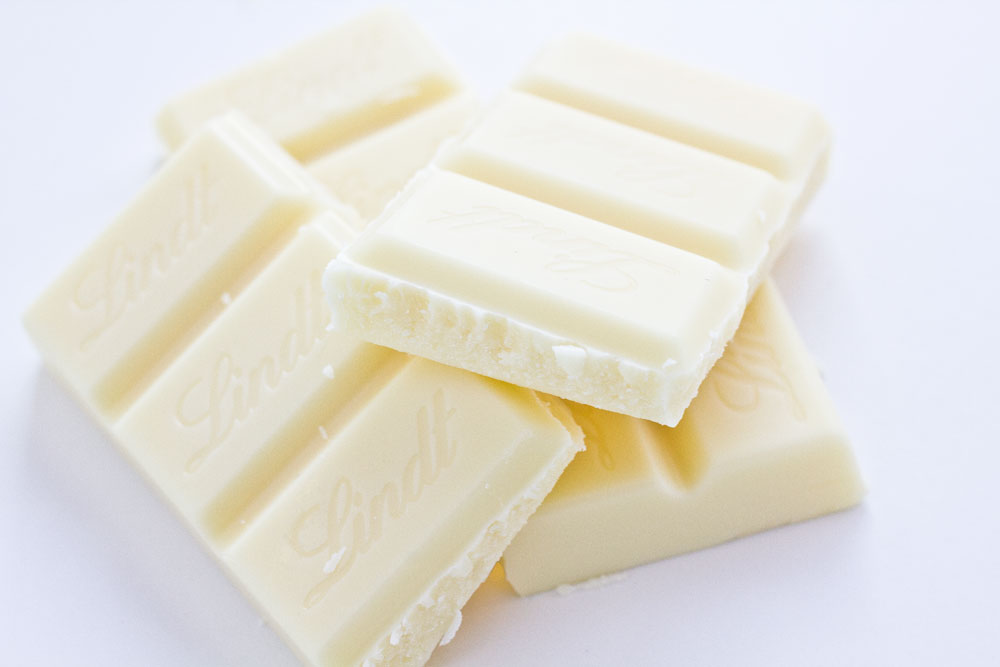
\includegraphics[width=\paperwidth]{whitechocolate}
\end{frame}

\begin{frame}
\centering
{\fontsize{60}{60}\selectfont THUNKS}
\end{frame}

\begin{frame}
\vspace*{8mm}
\centering
\small thunks 
\end{frame}

\begin{frame}
\centering

\includegraphics[height=\paperheight]{gift} 
\end{frame}

\begin{frame}
\hspace*{-11.2mm}
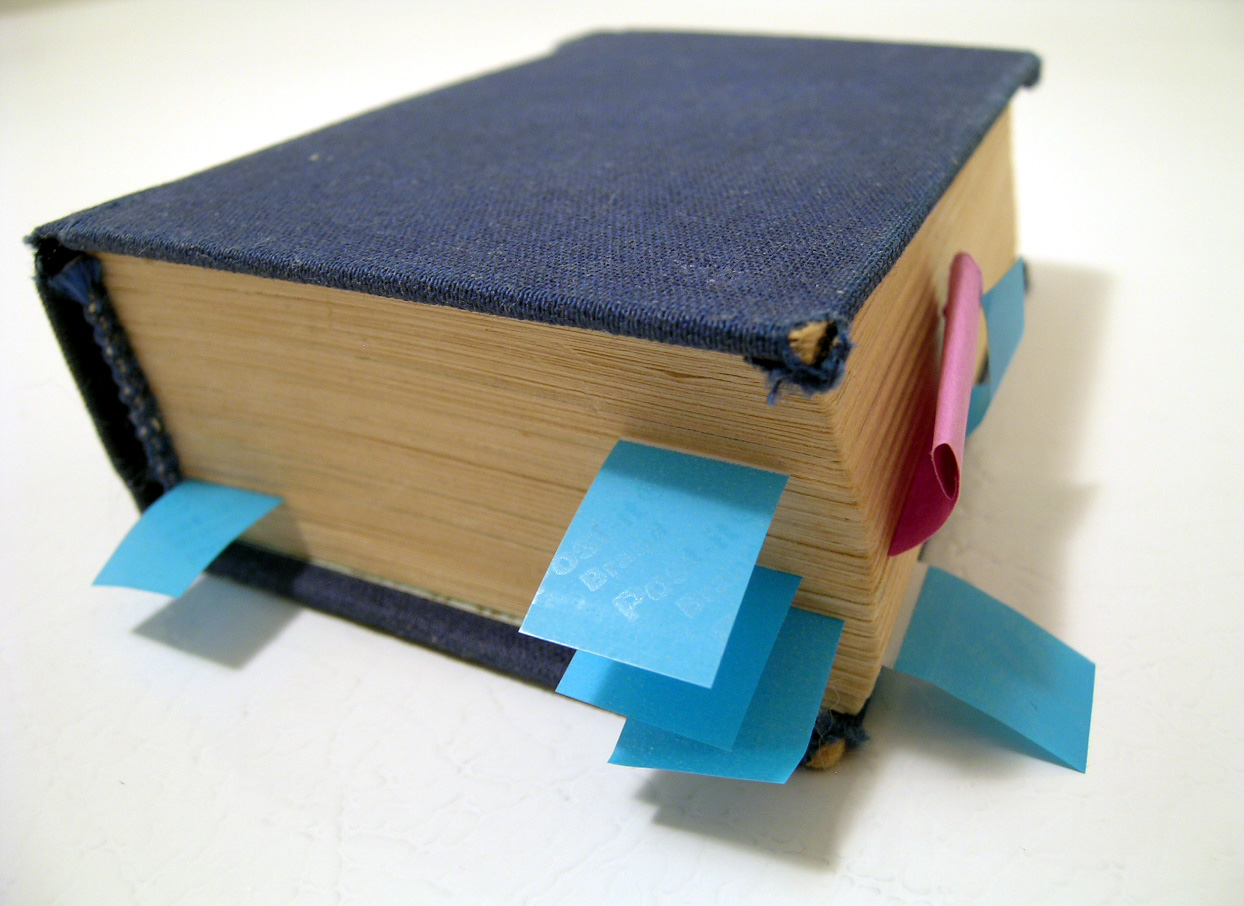
\includegraphics[width=\paperwidth]{bookmark}
\end{frame}

\begin{frame}[fragile]
\frametitle{Tradeoff}
\begin{center}
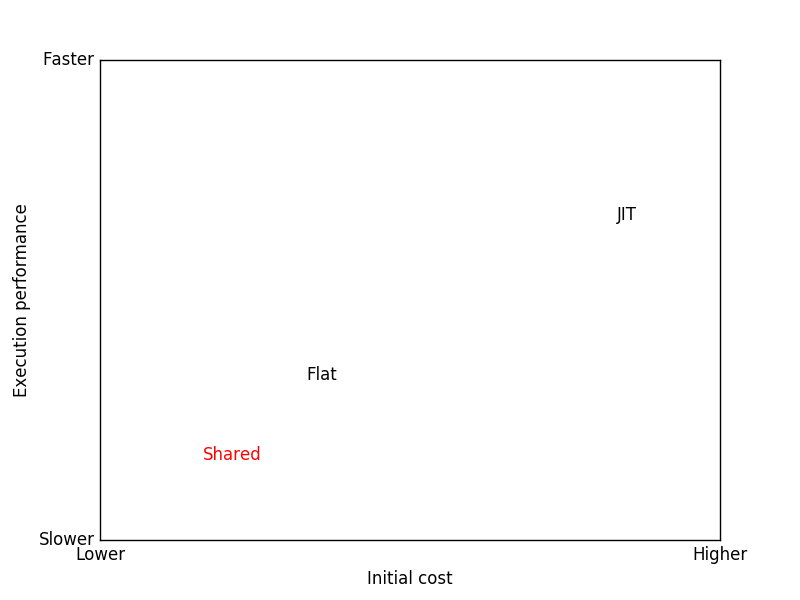
\includegraphics[width=10cm]{tradeoffplot}
\end{center}
\end{frame}

\sectionslide{\ce Machine}
{Simplicity is the final achievement.}
{Chopin}

\begin{frame}{Big Step \ce} 
\begin{align*}
\tag{App} \inference
{(m[l], \mu) \downarrow (\lambda b[l'], \mu') \quad f \not \in \textnormal{dom}(\mu') \\ 
(b[f], \mu'[f \mapsto n[l] \cdot l']) \downarrow v}
{(m \; n[l], \mu) \downarrow v}  
\end{align*}
\begin{align*}
\tag{Var} \inference
{\mu(l, i) = l_1 \mapsto c \cdot l_2 \quad (c, \mu) \downarrow (v, \mu')}
{(i[l],\mu) \downarrow (v, \mu'[l_1 \mapsto v \cdot l_2])}
\end{align*}
\end{frame}

\begin{frame}[fragile]
\frametitle{Small Step \ce}
\footnotesize
\begin{align*}
\tag{Closure} c &\Coloneqq t \left[l\right] \\
\tag{Heap} \mu &\Coloneqq \epsilon \; | \; \mu \left[ l \mapsto \rho \right] \\
\tag{Environment} \rho &\Coloneqq \bullet \; | \; c \cdot l \\
\tag{Stack} \sigma &\Coloneqq \square \; | \; \sigma \; c \;  | \; \sigma \; u \\
\langle v,  \sigma \; u , \mu \rangle 
  &\rightarrow
\langle v, \sigma, \mu\left(u \mapsto v \cdot l\right) \rangle  
\; \textnormal{where} \; c \cdot l = \mu\left(u\right) \\
\langle \lambda t\left[l\right], \sigma \; c, \mu \rangle 
  &\rightarrow
\langle t\left[f\right], \sigma, \mu\left[f \mapsto c \cdot l\right]\rangle f
\not \in \textnormal{dom}\left(\mu\right)  \\
\langle t \; t'\left[l\right], \sigma, \mu \rangle
  &\rightarrow
\langle t\left[l\right], \sigma \; t'\left[l\right], \mu \rangle \\
\langle i\left[l\right], \sigma, \mu \rangle
  &\rightarrow
\langle c, \sigma \; l'', \mu \rangle
\; \textnormal{where} \; l'' \mapsto c \cdot l' = \mu\left(l, i\right)
\end{align*}
\end{frame}

\begin{frame}{Example}
\begin{center}
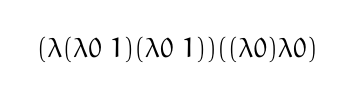
\begin{tikzpicture}
  \node (tm) at (0,0) {$(\lambda (\lambda 0 \; 1) (\lambda 0 \; 1))((\lambda 0) \lambda 0)$};
\end{tikzpicture}
\vskip0pt plus 1fill
\end{center}
$$(\lambda (\lambda 0 \; 1) (\lambda 0 \; 1))((\lambda 0) \lambda 0)$$
\end{frame}

\begin{frame}{Example (cont.)}
\begin{center}
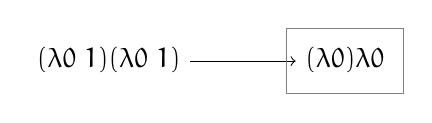
\begin{tikzpicture}
  \node (tm) at (0,0) {$(\lambda 0 \; 1) (\lambda 0 \; 1)$}; 
  \node (arg) at (3,0) {$(\lambda 0) \lambda 0$};
  \draw [->] (tm) -- (arg); 
  \node [style={rectangle, draw=black!50}, fit={(arg)}] {}; 
\end{tikzpicture}
\vskip0pt plus 1fill
\end{center}
$$(\lambda (\lambda 0 \; 1) (\lambda 0 \; 1))((\lambda 0) \lambda 0)$$
\end{frame}

\begin{frame}{Example (cont.)}
\begin{center}
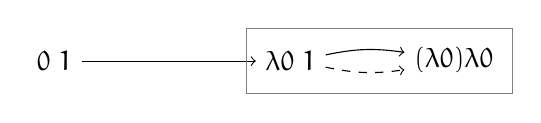
\begin{tikzpicture}[->]
  \node (tm) at (0,0) {$0 \; 1$}; 
  \node (arg1) at (3,0) {$\lambda 0 \; 1$}; 
  \node (arg) [right=of arg1.east] {$(\lambda 0) \lambda 0$};
  \path (tm) edge node [] {} (arg1);
  \path
    (arg1) edge [bend left=10] node  {} (arg);
  \path[dashed]
    (arg1) edge [bend right=10] node {} (arg);
  \node [style={rectangle, draw=black!50}, fit={(arg1) (arg)}] {}; 
\end{tikzpicture}
\vskip0pt plus 1fill
\end{center}
$$(\lambda (\lambda 0 \; 1) (\lambda 0 \; 1))((\lambda 0) \lambda 0)$$
\end{frame}

\begin{frame}{Example (cont.)}
\begin{center}
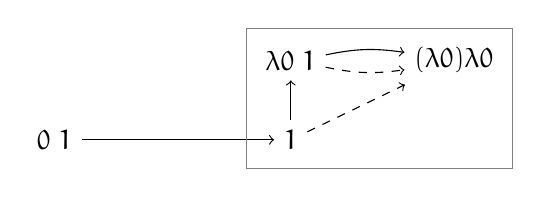
\begin{tikzpicture}[->]
  \node (tm) at (0,0) {$0 \; 1$}; 
  \node (arg2) at (3,0) {$1$}; 
  \node (arg1) at (3,1) {$\lambda 0 \; 1$}; 
  \node (arg) [right=of arg1.east] {$(\lambda 0) \lambda 0$};
  \path (tm) edge node {} (arg2);
  \path 
    (arg2) edge node {} (arg1)
    (arg1) edge [bend left=10]  node {} (arg);
  \path[dashed]
    (arg2) edge node {} (arg)
    (arg1) edge [bend right=10] node {} (arg);
  \node [style={rectangle, draw=black!50}, fit={(arg2) (arg1) (arg)}] {}; 
\end{tikzpicture}
\vskip0pt plus 1fill
\end{center}
$$(\lambda (\lambda 0 \; 1) (\lambda 0 \; 1))((\lambda 0) \lambda 0)$$
\end{frame}

\begin{frame}{Example (cont.)}
\begin{center}
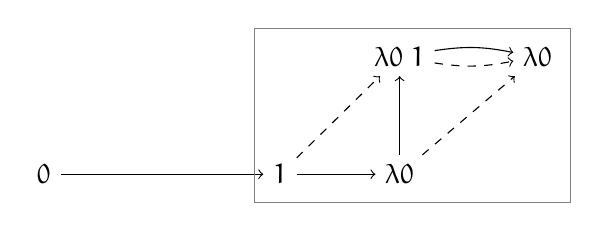
\begin{tikzpicture}[->]
  \node (tm) at (0,0) {$0$}; 
  \node (arg3) at (3,0) {$1$}; 
  \node (arg2) [right=of arg3.east] {$\lambda 0$}; 
  \node (arg1) [above=of arg2.north] {$\lambda 0 \; 1$}; 
  \node (arg) [right=of arg1.east] {$\lambda 0$};
  \path (tm) edge node {} (arg3);
  \path
    (arg3) edge node {} (arg2) 
    (arg2) edge node {} (arg1)
    (arg1) edge [bend left=10] node {} (arg);
  \path[dashed]
    (arg3) edge node {} (arg1) 
    (arg2) edge node {} (arg)
    (arg1) edge [bend right=10] node {} (arg);
  \node [style={rectangle, draw=black!50}, fit={(arg3) (arg2) (arg1) (arg)}] {}; 
\end{tikzpicture}
\vskip0pt plus 1fill
\end{center}
$$(\lambda (\lambda 0 \; 1) (\lambda 0 \; 1))((\lambda 0) \lambda 0)$$
\end{frame}

\begin{frame}{Example (cont.)}
\begin{center}
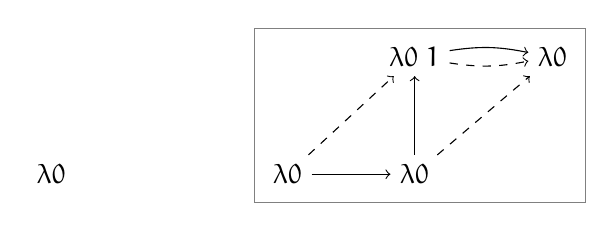
\begin{tikzpicture}[->]
  \node (tm) at (0,0) {$\lambda 0$}; 
  \node (arg3) at (3,0) {$\lambda 0$}; 
  \node (arg2) [right=of arg3.east] {$\lambda 0$}; 
  \node (arg1) [above=of arg2.north] {$\lambda 0 \; 1$}; 
  \node (arg) [right=of arg1.east] {$\lambda 0$};
  \path
    (arg3) edge node {} (arg2) 
    (arg2) edge node {} (arg1)
    (arg1) edge [bend left=10] node {} (arg);
  \path[dashed]
    (arg3) edge node {} (arg1) 
    (arg2) edge node {} (arg)
    (arg1) edge [bend right=10] node {} (arg);
  \node [style={rectangle, draw=black!50}, fit={(arg3) (arg2) (arg1) (arg)}] {}; 
\end{tikzpicture}
\vskip0pt plus 1fill
\end{center}
$$(\lambda (\lambda 0 \; 1) (\lambda 0 \; 1))((\lambda 0) \lambda 0)$$
\end{frame}

\sectionslide{Native Code Compiler}
{Yeah, I am lazy. There's no doubt about that.}
{Usain Bolt}

\begin{frame}
\frametitle{Implementation}
\footnotesize
\begin{align*}
\tag{Upd}
\langle v,  \sigma \; u , \mu \rangle 
  &\rightarrow
\langle v, \sigma, \mu\left(u \mapsto v \cdot l\right) \rangle  
\; \textnormal{where} \; c \cdot l = \mu\left(u\right) \\
\tag{Abs}
\langle \lambda t\left[l\right], \sigma \; c, \mu \rangle 
  &\rightarrow
\langle t\left[f\right], \sigma, \mu\left[f \mapsto c \cdot l\right]\rangle f
\not \in \textnormal{dom}\left(\mu\right)  \\
\tag{App}
\langle t \; t'\left[l\right], \sigma, \mu \rangle
  &\rightarrow
\langle t\left[l\right], \sigma \; t'\left[l\right], \mu \rangle \\
\tag{Var}
\langle i\left[l\right], \sigma, \mu \rangle
  &\rightarrow
\langle c, \sigma \; l'', \mu \rangle
\; \textnormal{where} \; l'' \mapsto c \cdot l' = \mu\left(l, i\right)
\end{align*}

\begin{align*}
\textmd{Upd} &\rightarrow \texttt{5 x64 Instructions} \\
\textmd{Abs} &\rightarrow \texttt{6 x64 Instructions} \\
\textmd{App} &\rightarrow \texttt{2 x64 Instructions} \\
\textmd{Var} &\rightarrow \texttt{6 x64 Instructions} \\
\end{align*}
\end{frame}

\begin{frame}[fragile]
\frametitle{Extensions}
\small
\begin{lstlisting}
data Expr a b = Var b 
              | Tail b
              | App (Expr a b) (Expr a b) 
              | Lam a (Expr a b)
              | Lit Literal
              | Op Op
              | World
\end{lstlisting}
\end{frame}

\begin{frame}[fragile]{Machine Operations}
\small
\begin{lstlisting}
data Op = Add | Sub | Mul | Div | Mod 
        | Eq | Neq | Lt | Gt | Le | Ge 
        | Write WordSize | Read WordSize 
        | Call String Int | Syscall Int 
\end{lstlisting}
\end{frame}

\begin{frame}[fragile]{Data Types}
\small
\begin{lstlisting}
# Booleans
false = \t.\f.f
true = \t.\f.t
and = \a.\b.(a b false)

# Lists
cons = \h.\t.\n.\c.(c h t)
nil = true

# Either 
Left = \v.\l.\r.(l v)
Right = \v.\l.\r.(r v)
\end{lstlisting}
\end{frame}

\begin{frame}[fragile]{Example Program}
\small
\begin{lstlisting}
gcd = (Y \gcd.\a.\b.(b = 0 
      a 
      (gcd b (a % b))))

main = (printf "%d" (gcd 25 10))
\end{lstlisting}
\end{frame}

\begin{frame}[fragile]{System Calls}
\begin{lstlisting}
sys_exit = \code.\w.[w 60 code 
  \a.\t.\w._!1]
sys_getpid = \w.[w 39 \t.\w._!0]
\end{lstlisting}
\end{frame}

\begin{frame}[fragile]
\frametitle{Results}
\centering
\textbf{Hypothesis:} Some programs can benefit from having lightweight thunks
despite the cost of slower variable dereferences.
\end{frame}

\begin{frame}
\frametitle{Results}
\begin{itemize}
\item Nofib benchmark suite (Integers)
\item Recursion: Y combinator
\item ADTs: Scott encodings
\item Times averaged over 5 runs
\end{itemize}
\end{frame}

\definecolor{lightgreen}{rgb}{0.8,1,0.8}
\definecolor{lightred}{rgb}{1,0.8,0.8}
\definecolor{lightgray}{rgb}{0.8,0.8,0.8}
\newcolumntype{g}{>{\columncolor{lightgray}}X}

\begin{frame}[fragile]
\frametitle{Results}
\centering
\small
\begin{tabularx}{\textwidth}{l | X | g | X}
& GHC & $\mathcal{CE}$ & UHC \\
\hline
\texttt{exp3 8} & 1.038 & 1.530 & 2.286 \\
\rowcolor{lightred}
\texttt{tak 16 8 0} & 0.006 & 0.366 & 1.416 \\
\rowcolor{lightgreen}
\texttt{primes 1500} & 0.230 & 0.256 & 1.532 \\
\texttt{queens 9} & 0.012 & 0.206 & 0.598 \\
\texttt{fib 35} &  0.110 & 2.234 & 8.342 \\
\texttt{digits-of-e1 1000} & 0.118 & 3.576 & 22.010 \\
\rowcolor{lightgreen}
\texttt{digits-of-e2 1000} & 0.372 & 0.404 & 3.278 \\
\texttt{fannkuch 8} & 0.048 & 0.560 & 2.196 
\end{tabularx}
\begin{center}
Wall clock times in seconds \\
\texttt{GHC} and \texttt{UHC} run with \texttt{-O3}
\end{center}
\end{frame}

\begin{frame}[fragile]
\frametitle{Church Numerals Results}
\centering
\small
\begin{tabularx}{\textwidth}{l | X | g | X}
& GHC & $\mathcal{CE}$ & UHC \\
\hline
\texttt{exp3 8} & N/A & N/A & N/A \\
\texttt{tak 14 7 0} & 1.016 & 1.610 & 7.782 \\
\texttt{primes 32} & 0.666 & 0.846 & 5.290 \\
\texttt{queens 8} & 0.154 & 0.242 & 1.508 \\
\texttt{fib 23} &  0.468 & 0.626 & 5.336 \\
\texttt{digits-of-e1 } & N/A & N/A & N/A \\
\rowcolor{lightgreen}
\texttt{digits-of-e2 6} & 0.670 & 0.138 & 5.534 \\
\texttt{fannkuch 7} & 0.040 & 0.142 & 0.808
\end{tabularx}
\begin{center}
Wall clock times in seconds \\
\texttt{GHC} and \texttt{UHC} run with \texttt{-O3}
\end{center}
\end{frame}

\sectionslide{Verified Compiler}
{A program without a specification cannot be incorrect, it can only be
surprising.}
{J. J. Horning}

\begin{frame}{Definition}
Machine checked proof that behaviour is preserved through compilation.
\end{frame}

\section{Compiler}

\begin{frame}[fragile]{Var}
\begin{lstlisting}
mov (EP%2) EP ; ... 
push EP ;
push 0 ;
mov (EP%1) EP ;
jump (EP%0)
\end{lstlisting}
\end{frame}

\begin{frame}[fragile]{App}
\begin{lstlisting}
push EP ;
push n ;
jump m 
\end{lstlisting}
\end{frame}

\begin{frame}[fragile]{Upd}
\begin{lstlisting}
pop R1 ;
mov v (R1%0) ;
mov EP (R1%1) ;
jump v 
\end{lstlisting}
\end{frame}

\begin{frame}[fragile]{Take}
\begin{lstlisting}
new 3 R2 ;
mov R1 (R2%0) ;
pop (R2%1) ;
mov EP (R2%2) ;
mov R2 EP ;
jump b
\end{lstlisting}
\end{frame}

\section{Specification}
\begin{frame}{Input Semantics}
\begin{align*}
\tag{App} \inference
{(m[l], \mu) \downarrow (\lambda b[l'], \mu') \quad f \not \in \textnormal{dom}(\mu') \\ 
(b[f], \mu'[f \mapsto n[l] \cdot l']) \downarrow v}
{(m \; n[l], \mu) \downarrow v}  
\end{align*}
\begin{align*}
\tag{Var} \inference
{\mu(l, i) = l_1 \mapsto c \cdot l_2 \quad (c, \mu) \downarrow (v, \mu')}
{(i[l],\mu) \downarrow (v, \mu'[l_1 \mapsto v \cdot l_2])}
\end{align*}
\end{frame}

\begin{frame}{Correctness Specification}
\begin{theorem} 
If a term $t$ placed into the initial configuration for the big-step semantics
evaluates to a value configuration $v$, then the instruction machine starting
in the initial state with \texttt{compile 0 t} as its program will evaluate to a
related state $v'$.  
\end{theorem}
\end{frame}

\begin{frame}{Relation to Existing Semantics}
\begin{theorem}
If a closure $c$ in Curien's call-by-name semantics is equivalent to a
configuration $c'$, and $c$ steps to $v$, then there exists a $v'$ that our
call-by-name semantics steps to from $c'$ that is equivalent to $v$.
\end{theorem}
\end{frame}

\begin{frame}{Proof Thoughts}
\begin{itemize}
\item Preserving properties through heap mutation is hard.
\item Choose your induction hypotheses to be as general as possible.
\end{itemize}
\end{frame}

\sectionslide{Conclusion}
{No book can ever be finished. While working on it we learn just enough to find
it immature the moment we turn away from it.}
{Karl Popper}

\begin{frame}[fragile]{Half Verified?}
\begin{center}

\includegraphics[width=0.6\linewidth]{half-true}
\end{center}
\end{frame}

\begin{frame}[fragile]{Time and Space}
\begin{center}
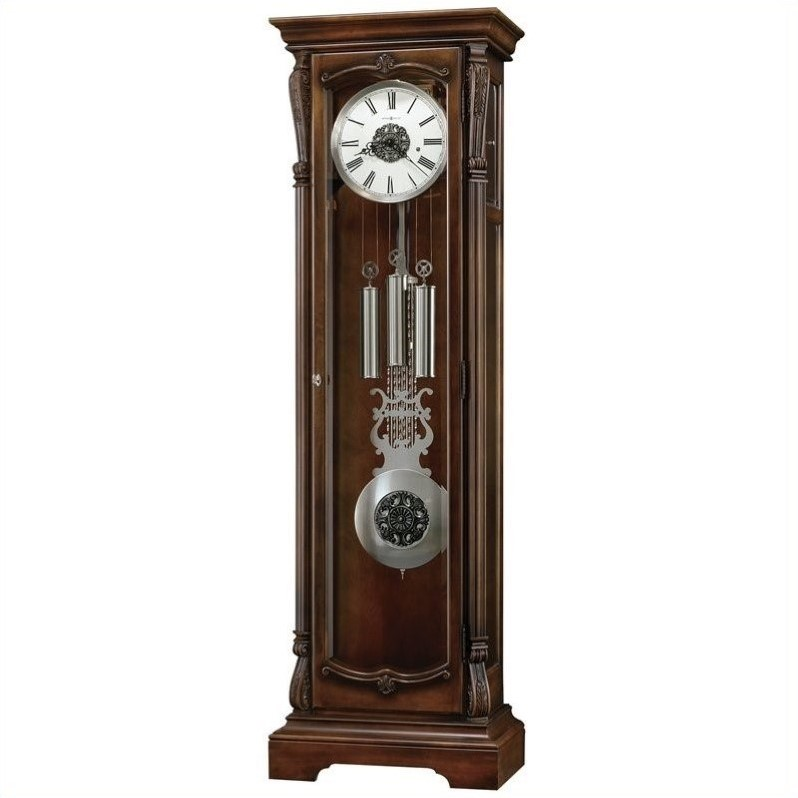
\includegraphics[width=0.4\linewidth]{time}
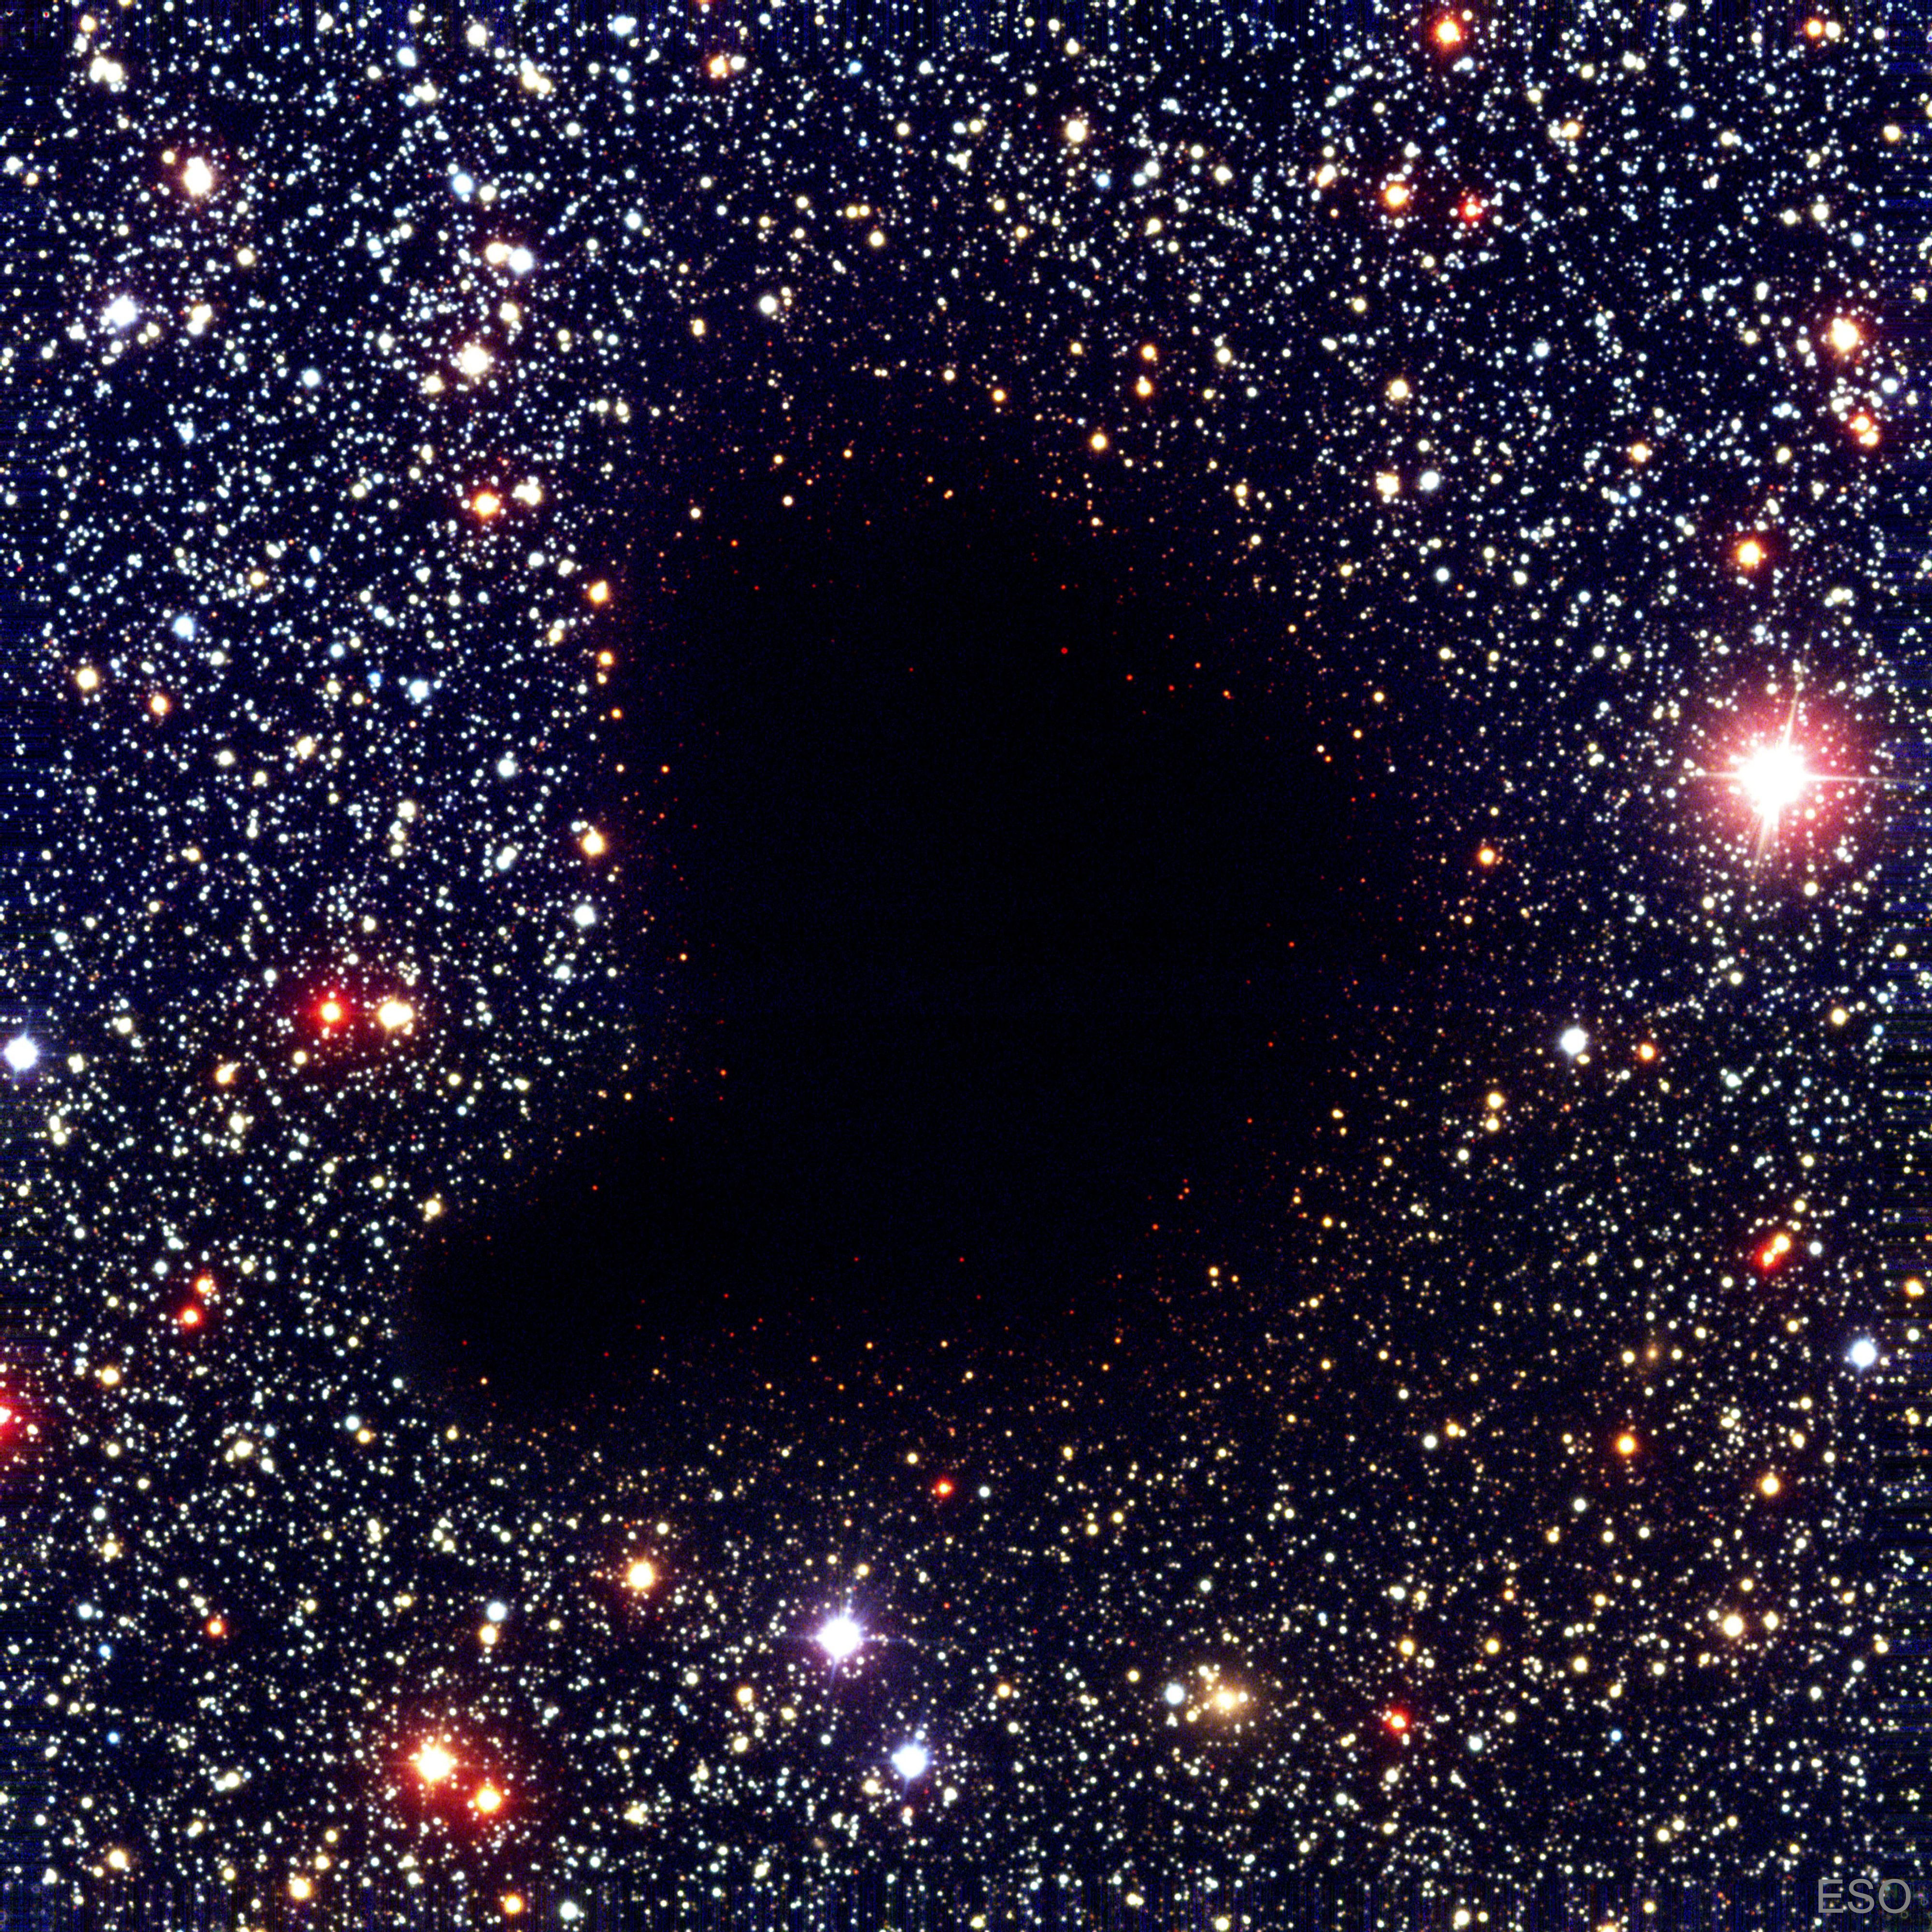
\includegraphics[width=0.4\linewidth]{space}
\end{center}
\end{frame}

\begin{frame}
\frametitle{Integration}
\centering

\includegraphics[width=5cm]{haskell}
\begin{itemize}
\item Shared + Flat
\item GHC Modifications
\item Optimizations 
\end{itemize}
\end{frame}

\begin{frame}
\frametitle{Parallelism}
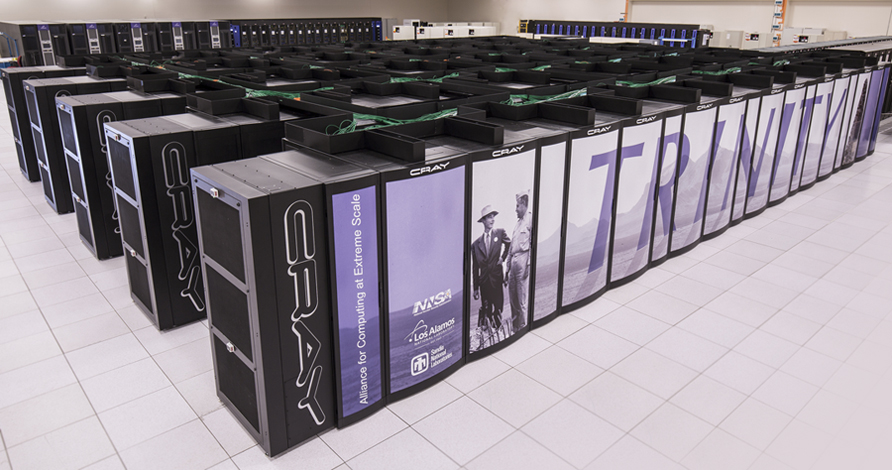
\includegraphics[width=7cm]{trinity}
\centering
\begin{itemize}
\item Lightweight threads
\item Lower overhead
\end{itemize}
\end{frame}

\section{Conclusion}
\begin{frame}{Final Thoughts}
\begin{itemize}
\item Lazier lazy evaluation
\item Promising performance 
\item First verified compiler for Call-by-Need
\item Still a lot to prove!
\end{itemize}
\end{frame}

\section{Thanks!}

%\appendix
%\begin{frame}{References}
%\nocite{*}
%\bibliography{demo_bibliography}
%\bibliographystyle{plain}
%\end{frame}

\end{document}
